% Prämabel
\documentclass[11pt,a4paper]{article}

% Codage
\usepackage[utf8]{inputenc}
\usepackage[T1]{fontenc}
\usepackage{siunitx}
\usepackage{indentfirst}

% Langue
\usepackage[english]{babel}

% Supplément
\usepackage{amsmath,amsfonts,amssymb}
\usepackage{verbatim} % pour faire des commentaires avec \begin{comment}...
\usepackage{float} % pour positioner un image exacetement où on veut
\usepackage
  [separate-uncertainty = true,
  multi-part-units = repeat]
  {siunitx} % Exemple \SI{0}{\kg \cdot \m^{-3}}

% Images
\usepackage[pdftex]{graphicx}
\usepackage{graphics}
\usepackage{subcaption} % pour positioner des figures côte à côte
\usepackage{wrapfig}

% pour l'inclusion de liens dans le document 
\usepackage[colorlinks,bookmarks=false,linkcolor=blue,urlcolor=blue]{hyperref}


% la mise en page
\usepackage{geometry}
\paperheight=297mm
\paperwidth=210mm

\pagestyle{plain}



% nouvelles commandes LaTeX, utilis\'ees comme abreviations utiles
\newcommand{\mail}[1]{{\href{mailto:#1}{#1}}}
\newcommand{\ftplink}[1]{{\href{ftp://#1}{#1}}}

%%%%%%%%%%%%%%%%%%%%%%%%%%%%%%%%%%%%%%%%%%%%%%%%%%%%%%%%
\begin{document}


% Le titre, l'auteur et la date
\title{Numerical Exercise \#3}
\author{XXX YYYY\\  % \\ pour fin de ligne
}
\date{\today}
\maketitle
%%%%%%%%%%%%%%%%%%%%%%%%%%%%%%%%%%%%%%%%%%%%%%%%%%%%%%%%



\newpage
\section{Question \#1 Numerical formulation}

Using the laplace operator, that was implemented in the previous exercises
$$
\triangle \phi_{i} = \frac{1}{dx^2}(\phi_{i+1}- 2\phi_{i} + \phi_{i-1})
$$
the diffusion equation with downscattering and fission can be expressed at any point inside of the material as

\begin{align}
D_{1}\triangle\phi_{1}-\Sigma_{af}\phi_{1} - \Sigma_{1\to2} \phi_1 & = -\frac{1}{k}(\nu \Sigma_{f_{1}}\phi_{1} + \nu \Sigma_{f_{2}}\phi_{2}) \\
D_{2} \triangle\phi_{2} - \Sigma_{as}\phi_{2} + \Sigma_{1\to_{2}} \phi_{2}  & = 0
\end{align}

where $\phi_{1}$ and $\phi_{2}$ are understood to be at point $i$.
The two equations can be organized in this matrix.
$$
\begin{pmatrix}
D_{f} \triangle - \Sigma_{af} - \Sigma_{1\to2}  & 0 \\
\Sigma_{1\to2}  & D_{s} \triangle - \Sigma_{as}
\end{pmatrix} \begin{pmatrix}
\phi_{f} \\
\phi_{s}
\end{pmatrix} = -
\frac{1}{k} \begin{pmatrix}
\nu\Sigma_{ff}  & \nu\Sigma_{fs} \\
0 & 0
\end{pmatrix} \begin{pmatrix}
\phi_{f} \\
\phi_{s}
\end{pmatrix}
$$


% Relationship between $\mathrm{\Phi}_i,\ \mathrm{\Phi}_{i+1},\ \mathrm{\Phi}_{i-1}$ for group g at any point within the material:
% \begin{equation}
% 	A \Phi_i + B \Phi_{i-1} +C \Phi_{i+1} = D
% \end{equation}

% Expression of the source term for the fast and thermal energy group:
% \begin{equation}
% 	b_1=...
% 	b_2=...
% \end{equation}
\section{Question \#2 Analytical solution for the bare system}

We make a seperation of variables, seperating $\phi_{g}(x)$ into an energy independant $\phi(x)$ and an energy group $g$ dependant amplitude $\varphi_{g}$:
$$
\phi_{g}(x) = \varphi_{g}\phi(x)
$$
then using that
$$
\triangle \phi(x) = B\phi(x)
$$
we can rewrite the equation
$$
\begin{pmatrix}
D_{s} B - \Sigma_{af} - \Sigma_{1\to2}  & 0 \\
\Sigma_{1\to2}  & D_{f} B - \Sigma_{as}
\end{pmatrix} \begin{pmatrix}
\varphi_{f} \\
\varphi_{s}
\end{pmatrix} = -
\frac{1}{k} \begin{pmatrix}
\nu\Sigma_{ff}  & \nu\Sigma_{fs} \\
0 & 0
\end{pmatrix} \begin{pmatrix}
\varphi_{f} \\
\varphi_{s}
\end{pmatrix}
$$
which is $A\varphi = \frac{F}{k}\varphi$
since A is a 2x2 matrix it can be easily inverted:
$$
A^{-1} = \frac{1}{\det(A)} \begin{pmatrix} (D_{f} B - \Sigma_{as}) & 0 \\ -\Sigma_{1\to2} & D_{s} B - \Sigma_{af} - \Sigma_{1\to2} \end{pmatrix}
$$
The determinant of \( A \) is given by:
$$
\det(A) = (D_{s} B - \Sigma_{a} - \Sigma_{1\to2})(D_{f} B - \Sigma_{a}) 
$$

\begin{equation}
	M = A^{-1} F=\frac{1}{\operatorname{det}(A)}\left(\begin{array}{cc}
	\left(D_f B-\Sigma_{a s}\right) \nu \Sigma_{f f} & \left(D_f B-\Sigma_{a s}\right) \nu \Sigma_{f s} \\
	-\Sigma_{1 \rightarrow 2} \nu \Sigma_{f f} & -\Sigma_{1 \rightarrow 2} \nu \Sigma_{f s}
	\end{array}\right)
\end{equation}

The eigenvector of this matrix M can be found using numerical comutations. 
% You need to find an eigenvector, stupid XD
% \[
% \varphi = A^{-1} \left( -\frac{1}{k} F \varphi \right).
% \]

% Perform the multiplication:
% \[
% \varphi = \frac{1}{\det(A)}
% \begin{pmatrix} 
% (D_f B - \Sigma_{as}) \left(-\frac{1}{k} (\nu \Sigma_{ff} \varphi_f + \nu \Sigma_{fs} \varphi_s)\right) \\ 
% -\Sigma_{1 \to 2} \left(-\frac{1}{k} (\nu \Sigma_{ff} \varphi_f + \nu \Sigma_{fs} \varphi_s)\right) 
% \end{pmatrix}.
% \]

% This gives:
% \[
% \varphi_f = \frac{-1}{k \det(A)} (D_f B - \Sigma_{as}) (\nu \Sigma_{ff} \varphi_f + \nu \Sigma_{fs} \varphi_s),
% \]
% \[
% \varphi_s = \frac{\Sigma_{1 \to 2}}{k \det(A)} (\nu \Sigma_{ff} \varphi_f + \nu \Sigma_{fs} \varphi_s).
% \]


\begin{equation}
	k_{eff}=1.0843329711143195
\end{equation}


keff (scientific format with 5 significant digits): \\

\section{Question \#3 Numerical solution of the bare homogeneous reactor}



keff (scientific format with 5 significant digits): 0.0314159\\

fast buckling (scientific format with 5 significant digits):0.03135 \\

thermal buckling (scientific format with 5 significant digits): 0.03135\\

analytical buckling : 0.03141

\begin{figure}[h]
	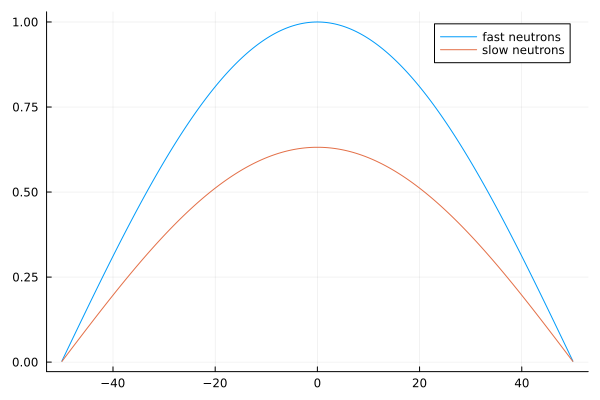
\includegraphics[width=7cm]{../../figs/ex3/bare.png}
	\centering
	\caption{Fast and thermal fluxes in the bare reactor for a mesh size of 0.1 cm.}
\end{figure}

\section{Question \#4}
\begin{figure}[h]
	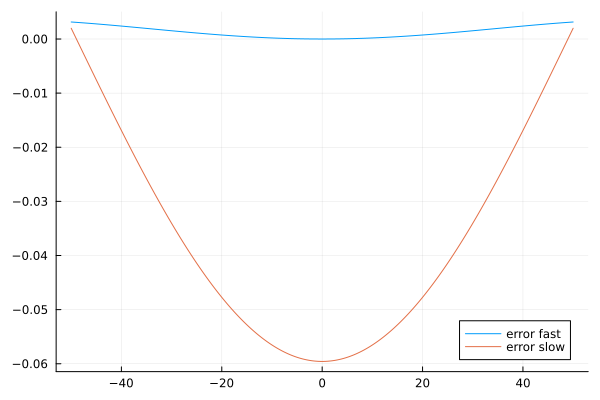
\includegraphics[width=7cm]{../../figs/ex3/error.png}
	\centering
	\caption{Difference between numerical and analytical solutions for the fast and thermal fluxes in the bare reactor for a mesh size of 0.1 cm.}
\end{figure}

\section{Question \#5 Numerical solution of the reflected reactor}


keff (scientific format with 5 significant digits): \\

fast net current (scientific format with 5 significant digits) at the core/reflector interface: \\

thermal net current (scientific format with 5 significant digits) at the core/reflector interface: \\

\begin{figure}[h]
	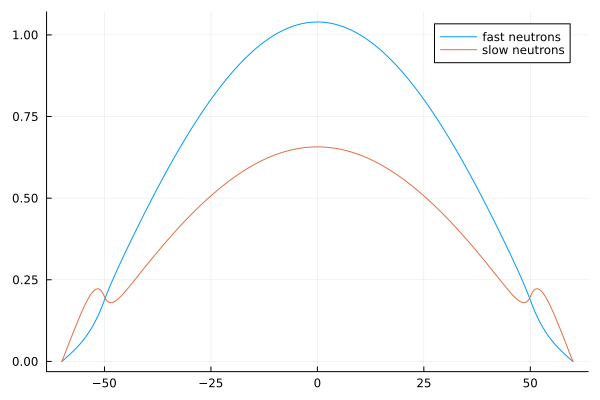
\includegraphics[width=7cm]{../../figs/ex3/reflected.png}
	\centering
	\caption{Fast and thermal fundamental fluxes in the reflected reactor for a mesh size of 0.1 cm.}
\end{figure}

\begin{figure}[h]
	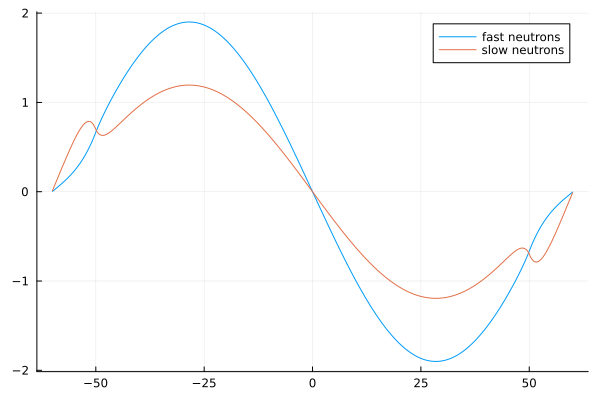
\includegraphics[width=7cm]{../../figs/ex3/fist_harmonic_reflected.png}
	\centering
	\caption{Fast and thermal first harmonic of the fluxes in the reflected reactor for a mesh size of 0.1 cm.}
\end{figure}

% k = (eigvals(M))[end - 1] = 1.0201735954627198 + 0.0im
% k = (eigvals(M))[end] = 1.0917083547920865 + 0.0im

keff (scientific format with 5 significant digits): \\

first harmonic eigenvalue (scientific format with 5 significant digits): \\



%%%%%%%






\end{document}
